
% This LaTeX was auto-generated from MATLAB code.
% To make changes, update the MATLAB code and republish this document.


    
    

\subsection*{fmincon options}

\begin{itemize}
\setlength{\itemsep}{-1ex}
   \item Algorithm: interior-point
   \item Display: iter
   \item GradObj: on
   \item GradConstr: on
   \item Hessian: user-supplied
   \item HessFcn:
   \item TolCon: $1e-06$
   \item TolFun: $1e-06$
   \item TolX: $1e-10$
\end{itemize}


\subsection*{Gitter und Intervallaenge}

\begin{itemize}
\setlength{\itemsep}{-1ex}
   \item Intervallaenge: 50
\end{itemize}


\subsection*{Environment}

\begin{par}
Anfangsbedingung:
\end{par} \vspace{1em}


\subsection*{Quadrocopter Eigenschaften}

\begin{itemize}
\setlength{\itemsep}{-1ex}
   \item States: $13$
   \item Controls: $4$
   \item Traegheitsmatrix:
   \item Gesamtmasse: $1.022$
   \item kT: $1.5e-07$
   \item kQ: $3e-09$
   \item d: $0.22$
   \item motor\_m: $0.075$
   \item motor\_r: $0.015$
\end{itemize}


\subsection*{Ergebnis}

\begin{par}

\begin{itemize}
   \item Zeit: $80.0083$
   \item Exitflag: $-2$
   \begin{itemize}
      \item  1: First-order optimality measure was less than options
      TolFun and maximum constraint violation was less than options
      TolCon
      \item  0: Number of iterations exceeded options MaxIter or
      number of function evaluations exceeded options MaxFunEvals.
      \item -2: No feasible point was found.
   \end{itemize}
   \item Iterations: $31$
\end{itemize}

\end{par} \vspace{1em}


\subsection*{Beispiel: Norm of Quaternionen}


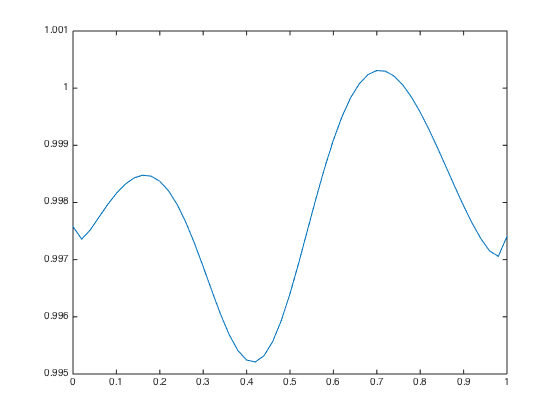
\includegraphics [width=4in]{rtoptmain_publish_01.png}
